\documentclass{article}
\usepackage[margin=1in]{geometry}
\usepackage{setspace}
\usepackage{amsmath}
\usepackage{amssymb}
\usepackage{physics}
\usepackage{graphicx}
\usepackage{relsize}

\title{Math 132 Final}
\author{Jiaping Zeng}
\date{12/13/2020}

\begin{document}
\setstretch{1.5}

\newpage
\begin{itemize}
      \item [P2] Find and plot all $z\in\mathbb{C}$ such that $z^3=-1$.\\
            \textbf{Answer}: We have $z^3=-1\implies z^3=\cos\pi+i\sin\pi$, so by the $n$th roots formula, the roots are:\\
            $z_1=\cos\frac{\pi}{3}+i\sin\frac{\pi}{3}=\frac{1}{2}+\frac{\sqrt{3}}{2}i$\\
            $z_2=\cos(\frac{\pi}{3}+\frac{2\pi}{3})+i\sin(\frac{\pi}{3}+\frac{2\pi}{3})=-1$\\
            $z_3=\cos(\frac{\pi}{3}+\frac{4\pi}{3})+i\sin(\frac{\pi}{3}+\frac{4\pi}{3})=\frac{1}{2}-\frac{\sqrt{3}}{2}i$
            \begin{center}
                  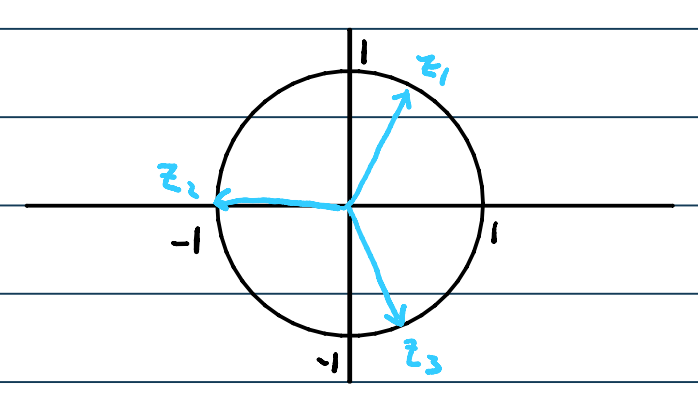
\includegraphics[width=3in]{p2.png}
            \end{center}
\end{itemize}

\newpage
\begin{itemize}
      \item [P4] Define $u:\mathbb{R}^2\rightarrow\mathbb{R}$ by $u(x,y)=4x^3y-4y^3x-2x$.
            \begin{itemize}
                  \item [(a)] Show that $u$ is a harmonic function.\\
                        \textbf{Answer}: We have $u_x=12x^2y-4y^3-2$ and $u_y=4x^3-12xy^2$, then $u_{xx}=24xy$ and $u_{yy}=-24xy$. Then $\Delta u=u_{xx}+u_{yy}=0$ and therefore $u$ is harmonic.
                  \item [(b)] Find a harmonic conjugate $v$ for $u$.\\
                        \textbf{Answer}: By Cauchy-Riemann, $v$ must satisfy $u_x=v_y\implies v=\int 12x^2y-4y^3-2dy=-y^4+6y^2x^2-2y+C(x)\implies v_x=12xy^2+C'(x)$. Again by Cauchy-Riemann, $v$ must also satisfy $u_y=-v_x\implies v_x=-4x^3+12xy^2$. Then we have $C'(x)=-4x^3\implies C(x)=-x^4$ and therefore $v(x,y)=-y^4+6y^2x^2-2y-x^4$ by substitution.
            \end{itemize}
\end{itemize}

\newpage
\begin{itemize}
      \item [P6]
            \begin{itemize}
                  \item [(a)] Find $\dfrac{1}{2\pi i}\mathlarger{\int_{C_2(0)}}\dfrac{[\Re(z)]^2}{z}dz$.\\
                        \textbf{Answer}: We have $\gamma(t)=2e^{it}$ for $t\in[0,2\pi]$, then $\mathlarger{\int_{C_2(0)}}\dfrac{[\Re(z)]^2}{z}dz=\mathlarger{\int_0^{2\pi}}f(\gamma(t))\gamma'(t)dt=\mathlarger{\int_0^{2\pi}}\dfrac{[\Re(2e^{it})]^2}{2e^{it}}\cdot 2ie^{it}dt=4i\mathlarger{\int_0^{2\pi}}\cos^2(t)dt=4\pi i$, so $\dfrac{1}{2\pi i}\mathlarger{\int_{C_2(0)}}\dfrac{[\Re(z)]^2}{z}dz=\dfrac{4\pi i}{2\pi i}=2$.
                  \item [(b)] Find $\mathlarger{\int_\gamma}\dfrac{2z+1}{e^{\pi z}-1}dz$, where $\gamma$ is the pictured path.\\
                        \textbf{Answer}: Let $f=\dfrac{2z+1}{e^{\pi z}-1}$. We can start by finding the singularities $f$ by solving $e^{\pi z}-1=0\implies z_0=0,2i$. Then, by Proposition $\bigstar$, we have simple poles at both $0$ and $2i$. We can now find their residues as follows:\\
                        $\Res(f,0)=\mathlarger{\lim_{z\rightarrow 0}}zf(z)=\mathlarger{\lim_{z\rightarrow 0}}\dfrac{z(2z+1)}{e^{\pi z}-1}=\dfrac{1}{\pi}$\\
                        $\Res(f,2i)=\mathlarger{\lim_{z\rightarrow 2i}}(z-2i)f(z)=\mathlarger{\lim_{z\rightarrow 2i}}\dfrac{(z-2i)(2z+1)}{e^{\pi z}-1}=\dfrac{1}{\pi}+\dfrac{4i}{\pi}$\\
                        Then by Residue Theorem, we have\\
                        $\mathlarger{\int_\gamma}f(z)dz=2\pi i\left(\dfrac{1}{\pi}+\dfrac{1}{\pi}+\dfrac{4i}{\pi}\right)=\dfrac{2\pi i(2+4i)}{\pi}=-8+4i$.
            \end{itemize}
\end{itemize}

\newpage
\begin{itemize}
      \item [P8] Use residue theory to show that $\mathlarger{\int_{-\infty}^\infty}\dfrac{\cos(2x)}{x^2+1}dx=\pi e^{-2}$.\\
            \textbf{Answer}: For $R>0$, let $\sigma_R$ be the part of $C_R(0)$ in the upper half plane and let $\gamma_R=[[-R,R],\sigma_R]$. Note that $\cos(2z)$ is unbounded, but we have $\cos(2x)=\Re(e^{2ix})$, meaning that we can first evaluate $\mathlarger{\int_{-\infty}^\infty}\dfrac{e^{2ix}}{x^2+1}dx$ and take the real part. Let $f(z)=\dfrac{e^{2iz}}{z^2+1}$, then we have $\mathlarger{\int_{\gamma_R}}f(z)dz=\mathlarger{\int_{[-R,R]}}f(z)dz+\mathlarger{\int_{\sigma_R}}f(z)dz$.\\
            We want to first show that $\mathlarger{\int_{\sigma_R}}f(z)dz\rightarrow 0$. Let $L=\text{length}(\sigma_R)=\pi R$. For $z$ on $\sigma_R$, we have $\abs{f(z)}=\abs{\dfrac{e^{2iz}}{z^2+1}}=\dfrac{\abs{e^{2iz}}}{\abs{z^2+1}}\leq\dfrac{e^{\Re(2iz)}}{|\abs{z}^2-1|}\leq\dfrac{e^0}{\abs{R^2-1}}=\dfrac{1}{R^2-1}=M$ for $R$ large enough. Then by ML-estimate, we have $\abs{\mathlarger{\int_{\sigma_R}}f(z)dz}\leq ML=\dfrac{\pi R}{R^2-1}\rightarrow 0$ as $R\rightarrow\infty$. Therefore $\mathlarger{\lim_{R\rightarrow\infty}\int_{\sigma_R}}f(z)dz=0$.
            We will now find $\mathlarger{\int_{\gamma_R}}f(z)dz$ using Residue Theorem. We have $f(z)=\dfrac{e^{2iz}}{z^2+1}=\dfrac{e^{2iz}}{(z-i)(z+i)}$; since $-i$ is not in $\gamma_R$, we only need to examine $z_0=i$, which is a simple pole by Proposition $\bigstar$. Then $\Res(f,i)=\mathlarger{\lim_{z\rightarrow i}}(z-i)f(z)=\mathlarger{\lim_{z\rightarrow i}}\dfrac{e^{2iz}}{(z+i)}=\dfrac{e^{-2}}{2i}$. By Residue Theorem, $\mathlarger{\int_{\gamma_R}}f(z)dz=2\pi i\Res(f,i)=\dfrac{2\pi ie^{-2}}{2i}=\pi e^{-2}$.\\
            Then by substitution we have $\mathlarger{\int_{\gamma_R}}f(z)dz=\mathlarger{\int_{[-R,R]}}f(z)dz+\mathlarger{\int_{\sigma_R}}f(z)dz\implies \pi e^{-2}=\mathlarger{\int_{[-R,R]}}f(z)dz+0\implies\mathlarger{\int_{[-R,R]}}f(z)dz=\pi e^{-2}\implies\mathlarger{\int_{-\infty}^\infty}\dfrac{e^{2iz}}{z^2+1}dz=\pi e^{-2}$. Now we can take the real part, which gives us $\mathlarger{\int_{-\infty}^\infty}\dfrac{\cos(2x)}{x^2+1}dx=\Re\left(\mathlarger{\int_{-\infty}^\infty}\dfrac{e^{2iz}}{z^2+1}dz\right)=\Re(\pi e^{-2})=\pi e^{-2}$.
\end{itemize}

\newpage
\begin{itemize}
      \item [P9] Use the argument principle to find the number of zeroes of $f(z)=z^5+z^4+4z^3+10z^2+9$ in the first quadrant.\\
            \textbf{Answer}: Let $R$ be sufficiently large such that all zeroes of $f(z)$ is enclosed by the curve $\gamma_R=[[0,R],\sigma_R,[iR,0]]$ as shown below:
            \begin{center}
                  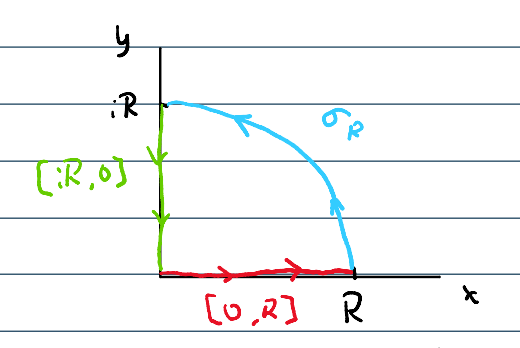
\includegraphics[width=3in]{p9-1.png}
            \end{center}
            Then, we have
            \begin{itemize}
                  \item [1.] $f([0,R])$: $f(x)=x^5+x^4+4x^3+10x^2+9$ for $x\in[0,R]$
                  \item [2.] $f(\sigma_R)$: $f(Re^{it})=R^5e^{5it}+R^4e^{4it}+4R^3e^{3it}+10R^2e^{2it}+9\approx R^5e^{5it}$ for $t\in[0,\frac{\pi}{2}]$
                  \item [3.] $f([iR,0])$: $f(iy)=iy^5+y^4-4iy^3-10y^2+9=(y^4-10y^2+9)+(y^5-4y^3)i$ for $y\in[0,R]$
            \end{itemize}
            Note that $f(z)\neq 0$ on $\gamma_R=[[0,R],\sigma_R,[iR,0]]$ since
            \begin{itemize}
                  \item [1.] $f(z)\geq 9$ on $[0,R]$
                  \item [2.] $R$ was chosen sufficiently large such that $f(z)\neq 0$ on $\sigma_R$
                  \item [3.] $f(iy)=(y^4-10y^2+9)+(y^5-4y^3)i=(y-3)(y-1)(y+1)(y+3)+y^3(y-2)(y+2)$; since $\Re f(iy)$ and $\Im f(iy)$ have no common zeroes, $f(z)\neq 0$ on $[iR,0]$
            \end{itemize}
            Now we can begin to sketch $f(\sigma_R)$. Since $f(x)$ always returns a real value for $x\in[0,R]$, $[0,R]$ maps to $[9,N]$ on the real axis where $N$ is some large number. Then, since $f(iR)=(R^4-10R^2+9)+(R^5-4R^3)i\approx R^4+R^5i\approx R^5i$, we also know that $\sigma_R$ ends at some point in the first quadrant, near the positive imaginary axis. Then since $f(Re^{it})\approx R^5e^{i(5t)},t\in[0,\frac{\pi}{2}]\implies 5t\in[0,\frac{5\pi}{2}]$, $\sigma_R$ is mapped to a circular path that wraps around the origin once and ends near the positive imaginary axis as shown below:
            \begin{center}
                  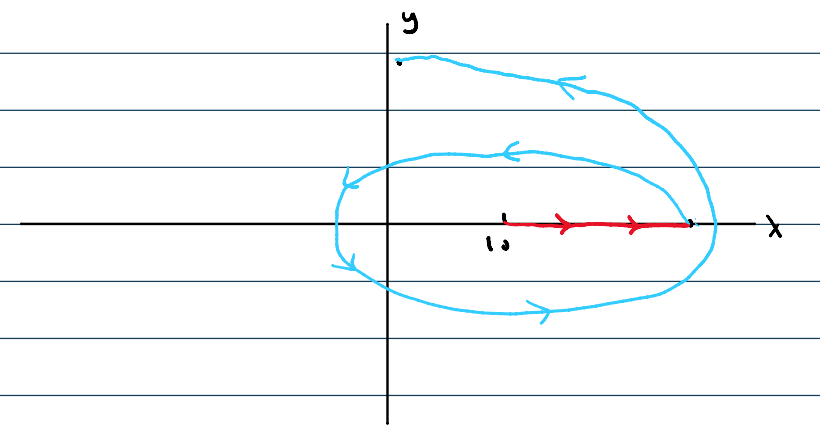
\includegraphics[width=4in]{p9-2.png}
            \end{center}
            We can now use a sign chart to find the map of $[iR,0]$:
            \begin{center}
                  \begin{tabular}{c|c|c|c|c}
                        \hline
                        $y=$        & $(0,1)$ & $(1,2)$ & $(2,3)$ & $(3,R)$ \\
                        \hline\hline
                        Quadrant    & IV      & III     & II      & I       \\
                        \hline\hline
                        $\Re f(iy)$ & +       & -       & -       & +       \\
                        \hline
                        $y-3$       & -       & -       & -       & +       \\
                        \hline
                        $y-1$       & -       & +       & +       & +       \\
                        \hline
                        $y+1$       & +       & +       & +       & +       \\
                        \hline
                        $y+3$       & +       & +       & +       & +       \\
                        \hline\hline
                        $\Im f(iy)$ & -       & -       & +       & +       \\
                        \hline
                        $y^3$       & +       & +       & +       & +       \\
                        \hline
                        $y-2$       & -       & -       & +       & +       \\
                        \hline
                        $y+2$       & +       & +       & +       & +       \\
                        \hline\hline
                  \end{tabular}
            \end{center}
            Therefore our $f(\gamma_R)$ looks like:
            \begin{center}
                  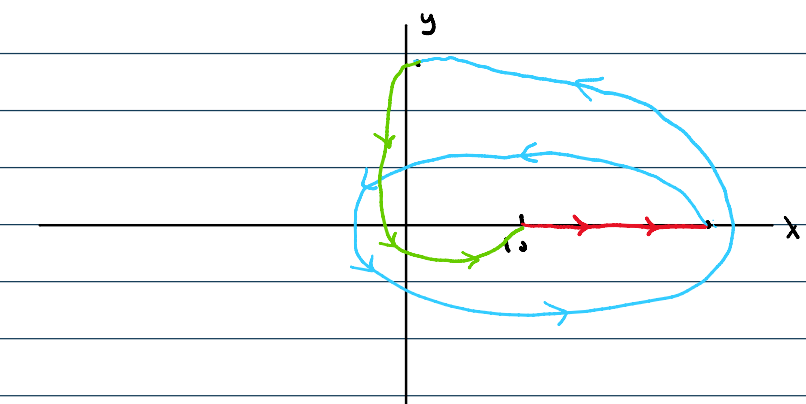
\includegraphics[width=4in]{p9-3.png}
            \end{center}
            So by the argument principle, since $f(\gamma_R)$ wraps counterclockwise around the origin twice, we have $N_0-N_\infty=2$. Since $f(z)$ is analytic, it has no poles, i.e. $N_\infty=0$. Therefore $N_0=2$, i.e. $f(z)$ has two zeroes in the first quadrant.
\end{itemize}

\newpage
\begin{itemize}
      \item [P11] Suppose that $f:A_{0,2}(0)\rightarrow\mathbb{C}$ is analytic and satisfies $f\left(\dfrac{1}{n}\right)=\dfrac{(-1)^n}{n^4}$ for $n=1,2,3,\ldots$. Show that there is a sequence $(z_n)_{n=1}^\infty$ with $z_n\rightarrow 0$ as $n\rightarrow\infty$ such that $f(z_n)\rightarrow 2020i$ as $n\rightarrow\infty$.\\
            \textbf{Answer}: Let $g(z)=\abs{z}^4$; since $f\left(\dfrac{1}{n}\right)=\dfrac{(-1)^n}{n^4}=\left(\dfrac{1}{n}\right)^4=g\left(\dfrac{1}{n}\right)$, we can define $z_n=e^{\ln\sqrt[4]{2020i}-i\pi n}$. Then clearly $z_n\rightarrow 0$ as $n\rightarrow\infty$ and we also have $g(z_n)\rightarrow 2020i$ as $n\rightarrow\infty$.
\end{itemize}

\newpage
I certify on my honor that I have neither given nor received any help, or used any non-permitted resources, while completing this evaluation.\\
Signature:
\includegraphics[width=2in]{signature.png}\\
Date: 12/13/2020


\end{document}